\chapter{Introduction}
\quad Parallel computing and software parallelization are the vast overlapping and complementary computer science areas with a history dating back to 1950s. With the advances in semiconductor industry the topics have left from high-end scientific supercomputers niche and spread to a much wider area spanning to all consumer electronic devices and are of major importance now. The parallelism is pervasive and all. Every computer scientist, software developer would benefit from having an insight into the area. Nonetheless the topics are extremely difficult and require a great deal of knowledge in various subtopics. Not all 

\section{The importance of parallel computing}
\label{parallel_computing_importance}
\quad The parallelism is pervasive and the future of computing is parallel. There are numerous factors which stress the importance of parallelism in modern computing.   

\begin{description}
\item[Abundance of natural parallelism] The field of High Performance Computing (HPC) has traditionally been concerned with scientific modelling and simulation of various natural phenomena (climate change, fluid flows, etc.). Such systems consist of numerous often independent parts. When we compile a highly parallel algorithm to a serial sequence of CPU instructions or process a huge data set with independent parts sequentially we are artificially constraining a vastly parallel computation to a serial one. Parallelism is not limited to a natural world, instead many algorithms have inherent parallelism in them.
\item[Semiconductor technology advances and power limits] With advances in transistor density it became possible to design more complicated CPUs. Initially the trend went into deeper pipelines, but running into power limits the industry design shifted towards multi core CPUs and multiprocessor systems. Such systems require of software to mirror the trend and become parallel.
\item[Domain inherent parallelism and specialized computations] The areas like computer graphics for instance have a lot of problems that can be processed in a Single Instruction Multiple Data (SIMD) fashion. That naturally led to specialized co-processors like GPUs. The hardware systems grow complex and heterogeneous.
\end{description}


\section{Challenges in Software Parallelization}
As section \ref{parallel_computing_importance} says, the parallelism in hardware has become pervasive. To achieve the full performance potential of modern hardware the software has to be mapped onto that parallel hardware. The process of software parallelization has characteristically been a very manual task, which is complex, time-consuming and error-prone.     

\subsection{Manual Parallelization Difficulties}
\quad Software parallelization has characteristically been manual. 
\begin{description}
\item[Problem understanding and partitioning]
\item[Communications and synchronization]
\item[Implementation and data dependencies]
\item[Performance analysis and tuning]
\end{description}

\subsection{Limitations of Automatic Techniques}
\quad There are various tools available to assist a programmer in the task of software parallelization. Parallelizing compilers are the most widely used.

Fully Automatic
The compiler analyzes the source code and identifies opportunities for parallelism.
The analysis includes identifying inhibitors to parallelism and possibly a cost weighting on whether or not the parallelism would actually improve performance. Loops are the most frequent target for automatic parallelization. Programmer Directed 
Using compiler directives or possibly compiler flags, the programmer explicitly tells the compiler how to parallelize the code. May be able to be used in conjunction with some degree of automatic parallelization also. The most common compiler generated parallelization is done using on-node shared memory and threads (such as OpenMP). If you are beginning with an existing serial code and have time or budget constraints, then automatic parallelization may be the answer. However, there are several important caveats that apply to automatic parallelization: Wrong results may be produced Performance may actually degrade Much less flexible than manual parallelization Limited to a subset (mostly loops) of code May actually not parallelize code if the compiler analysis suggests there are inhibitors or the code is too complex 

\begin{table}
  \begin{minipage}{\pagewidth}
  \begin{center}
    \begin{tabu}{M{3.0cm}M{1.0cm}M{3.0cm}M{1.0cm}M{3.0cm}M{1.0cm}}
      \hline
      \rowfont{\bfseries}
      reason & num & reason & num & reason & num\\\hline
      \textbf{unrecognised reduction} & 18 & \textbf{array privatization} & 7 & \textbf{AA conservativeness} & 60\\\hline
      \textbf{unknown iteration number} & 7 & \textbf{static dependencies} & 46 & \textbf{too complex} & 22\\\hline
      \textbf{uninlined calls} & 4 & \textbf{other} & 4 & \textbf{total} & 168\\\hline
    \end{tabu}
  \end{center}
  \end{minipage}
  \caption{Classification of loops missed by Intel Compiler for various reasons.}
  \label{tab:icc_missed_opportunities}
\end{table}%

We measured the running time of NASA Parallel Benchmarks after being compiled with Intel compiler (ICC) using various automatic parallelization options. Figure \ref{fig:benchmarks_runtime} illustrates the problems automatic parallelization has.

\begin{figure}[ht]
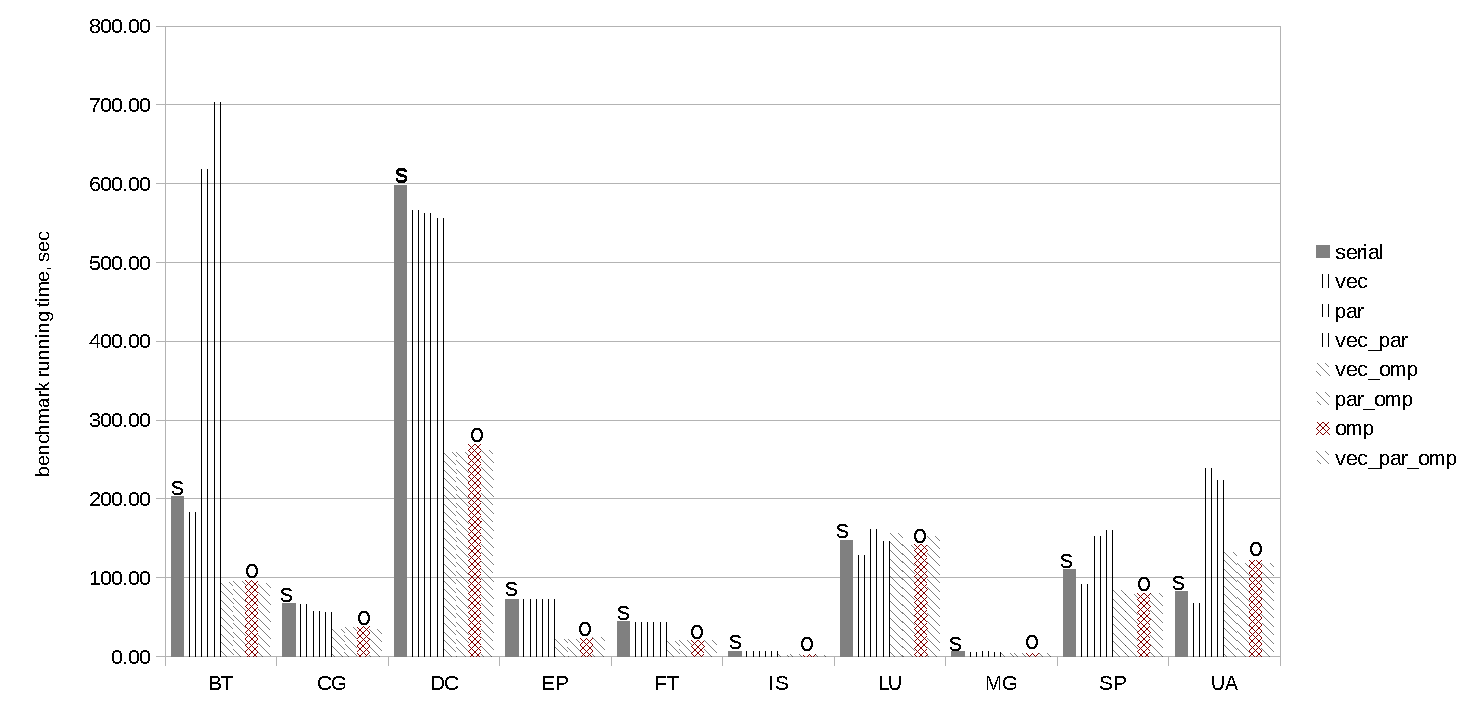
\includegraphics[width=1.0\textwidth]{images/benchmark_runtime.pdf}
\caption{The running time of various NPB benchmarks versions.}
\label{fig:benchmarks_runtime}
\end{figure}

\subsection{Limits of Machine Learning based methods}
\subsection{Data-Centric problem}
\subsection{Parallel Programming Models}
\quad With a number of various hardware vendors entering the market with their different hardware architectures the portability became a serious concern.  


the emergence of various hardware vendors, diffrent hardware architectures  

To combat the problem of software portability in the environment of growing number of different hardware architectures

\section{Software Parallelization Assistant}

\section{Computational Frameworks}
\quad In this work we propose an idea of computational frameworks. 


